% DRAFT of the SBS-stabilization-then-readout section for BB1GCR_note.tex.
% Insert before \section{Summary} (after the damage section's \FloatBarrier).
% METHODOLOGY paragraphs are final; RESULTS paragraphs marked <<FILL>> are completed
% from Paper_Data/sbs_authentic_sweep.npz once the sweep finishes.

\section{Reading an actively stabilized codeword: noisy SBS rounds before readout}\label{sec:sbs}

Section~\ref{sec:damage} let the codeword idle passively. A real logical memory does the
opposite: it is \emph{actively stabilized}, its lattice periodically re-sharpened by an
error-correction protocol that itself runs on the same imperfect hardware. The canonical GKP
stabilizer is the small--big--small (SBS) round of Royer \emph{et al.}\ and
Campagne-Ibarcq \emph{et al.}, realized on the Sivak \emph{et al.}\ device: a sequence of
conditional displacements interleaved with ancilla rotations that pumps entropy out of the
oscillator and pushes the state back toward the code manifold. But each round is a finite-duration
circuit coupling the oscillator to a lossy ancilla, so stabilization is a double-edged tool ---
it removes lattice error while injecting fresh decoherence. We ask how this trade-off interacts
with the readout: after $m$ rounds of \emph{noisy} SBS, how faithfully does each of the seven
protocols read the stabilized codeword, and how does that degrade as the rounds accumulate?

\paragraph{Model.} We use the authentic SBS implementation of the reference
device --- a $\sigma_z$-conditioned time evolution under the marker Hamiltonians
$\hat H_x=\hat\sigma_z\otimes a_1\hat x$ and $\hat H_p=-\hat\sigma_z\otimes a_1\hat p$, with an
$R_x(\pi/2)$ rotation conjugating the big step, acting on a finite-energy \emph{binomial} GKP
codeword ($\Delta=0.34$, $N_{\mathrm{cav}}=200$). The fresh $m=0$ codeword is the fixed point of
noiseless cooling: we run the stabilizer forward from vacuum for twenty rounds to obtain the
stabilized logical-$0$ state $G_{\mathrm{SBS},0}$, and take that as the input to the experiment.
A single SBS round of this implementation exchanges the two logical branches --- it is a stable
two-cycle, $G_{\mathrm{SBS},0}\!\leftrightarrow\!G_{\mathrm{SBS},1}$, with the fidelity returning
to $\gtrsim0.98$ after every second round --- so we sample an even number of rounds
$m\in\{0,2,4,6,8,10\}$, for which the encoding always returns to logical $0$ while having absorbed
the decoherence of $m$ physical stabilization circuits.\footnote{This parity exchange is a
convention of the reference implementation, not a defect: it is why the device's cooling
trajectory alternates between the $\mu=0$- and $\mu=1$-like states on consecutive iterations. Odd
$m$ would simply read the logical-$1$ branch of the same data.}

Noise enters the SBS rounds through the same collapse operators used throughout this note. During
the marker evolutions the master equation carries, according to the condition under test, transmon
decay $\sqrt{\gamma}\,\hat\sigma_-$ ($\gamma=1/200\,\mu\mathrm{s}^{-1}$), transmon dephasing
$\sqrt{\gamma_\phi/2}\,\hat\sigma_z$ ($\gamma_\phi=1/200\,\mu\mathrm{s}^{-1}$), oscillator photon
loss $\sqrt{\kappa}\,\hat a$ ($\kappa=1/1000\,\mu\mathrm{s}^{-1}$), or oscillator dephasing
$\sqrt{\kappa_\phi}\,\hat a^\dagger\hat a$ ($\kappa_\phi=1/5000\,\mu\mathrm{s}^{-1}$, the same
qualitative rate as in Sec.~\ref{sec:damage}). We run five separate stabilization experiments, one
per SBS-noise condition: \emph{all channels} together (transmon decay $+$ transmon dephasing $+$
oscillator loss), and each of transmon decay, transmon dephasing, oscillator decay, and oscillator
dephasing in isolation. In every experiment the stabilized state at each $m$ is then read out under
all six readout-circuit conditions of Sec.~\ref{sec:mesolve} --- noiseless, all channels, transmon
decay, transmon dephasing, oscillator decay, oscillator dephasing --- so that the SBS-noise axis
and the readout-noise axis are cleanly separated. As before we report the readout error $P(e)$ and
the post-read oscillator infidelity $1-F$ after the single calibrated corrective displacement,
against the pristine $m=0$ codeword; the analysis is for logical $0$.

\paragraph{A note on the vertical scale.} Because a genuine, non-collapsing SBS stabilizer is
available only in the device's native \emph{binomial}-GKP, $i=2$ quadrature convention, this
section uses that codeword rather than the Gaussian-comb encoding of
Secs.~\ref{sec:mesolve}--\ref{sec:damage}. The stabilized codeword is correspondingly softer than
the idealized comb --- even the freshly-cooled $m=0$ state reads at $P(e)\approx0.08$ under
noiseless pulses, the validated operating point of the reference SBS pipeline, rather than the
$\lesssim10^{-3}$ floors of Sec.~\ref{sec:mesolve}. The comparison of interest here is therefore
\emph{relative}: how each protocol and each noise channel move the operating point as the rounds
accumulate, not the absolute floor, which is set by the encoding rather than the readout gadget.

\paragraph{Heralding does not transfer to the stabilized codeword.} One protocol must be set
aside at the outset. Unlike the six deterministic protocols --- whose corrections are conditional
\emph{displacements} that act relative to the state and therefore inherit whatever lattice the
codeword carries --- the heralded scheme relies on a fixed, non-covariant momentum \emph{filter}
whose geometry is pinned to the Gaussian-comb lattice of Secs.~\ref{sec:mesolve}--\ref{sec:damage}.
On the binomial-GKP fixed point of the reference SBS pipeline, that filter is mis-registered: a
scan of the input displacement over a full two-cell window fails to bring the heralded readout below
$P(e)\approx0.47$ anywhere on the real axis, and momentum-axis displacements drive the
post-selection norm through zero (the heralding branch is rejected) rather than recovering it. In
other words, the heralded gadget would have to be re-derived from scratch for each encoding's
lattice; a rigid recalibration cannot rescue it. We therefore report the \emph{six deterministic}
protocols here and note only that the heralded scheme, alone among the seven, is not portable across
the encoding change --- a concrete cost of building readout around a lattice-specific measurement.

\paragraph{Noisy stabilization degrades readout slowly, and the ancilla is the culprit.}
Figure~\ref{fig:sbs} isolates the stabilization noise by reading every state under noiseless
pulses. All six protocols start from the same freshly-cooled floor, $P(e)\in[0.079,0.085]$ at
$m=0$, and rise gently and near-linearly as noisy rounds accumulate. The \emph{rate} of that rise
is set almost entirely by which channel is active during the SBS circuit, and the ordering is
sharp: transmon decay is by far the most damaging ($P(e)$ climbs $0.079\!\to\!0.097$ over ten
rounds), and the all-channels case tracks it almost exactly ($0.079\!\to\!0.098$), while
oscillator dephasing ($0.079\!\to\!0.086$), oscillator decay ($0.079\!\to\!0.083$) and transmon
dephasing ($0.079\!\to\!0.083$) each add only a few $\times10^{-3}$ over the whole sweep. That the
ancilla's $T_1$ dominates --- and that isolated oscillator loss is nearly harmless --- is exactly
what one expects of an actively-pumped stabilizer: the transmon is entangled with the oscillator
throughout each conditional displacement, so its decay corrupts the round it drives, whereas slow
photon loss is continually undone by the very map that injects it. Across the entire sweep the six
protocols stay bunched within a $\lesssim5\times10^{-3}$ band: once the codeword is being actively
stabilized, the choice of readout dressing matters far less than how many noisy rounds it has seen
and through which channel.

\paragraph{Readout noise adds a separable offset, and the shortest circuit wins.}
Figure~\ref{fig:sbs-readout} holds the stabilization at its realistic all-channels setting and
sweeps the readout circuit over its six noise conditions. Adding readout noise leaves the shape of
the $m$-dependence intact and shifts each protocol up by a nearly $m$-independent offset, so the two
noise axes are separable. But the offset is strongly \emph{protocol}-dependent, and it tracks the
\emph{duration} of the readout circuit rather than its correction content: single GCR --- the
shortest deterministic sequence, one pre-correction and one kick --- is almost immune, its $P(e)$
rising by only $+2.5\times10^{-3}$ under all-channels readout, while the five longer circuits are
lifted \emph{together} by $+1.8$ to $+2.0\times10^{-2}$, whether or not they carry detuning
corrections (bare BB1, with none, is lifted as much as the detuning-heavy schemes). Readout noise
therefore does not blur the family uniformly; it drives single GCR clearly below the pack and
widens the protocol band from $\sim6\times10^{-3}$ under noiseless pulses to $\sim2\times10^{-2}$.
The offset again follows the transmon --- all-channels and transmon-decay readout dominate
($\approx1.6$ and $0.9\times10^{-2}$ on average), oscillator decay contributes least
($\lesssim3\times10^{-3}$) --- reproducing the verdict of Sec.~\ref{sec:damage}: under
readout-circuit noise the least-exposed, shortest protocol is the most accurate, and the elaborate
corrections pay for their length.

\begin{figure}[tbp]
\centering
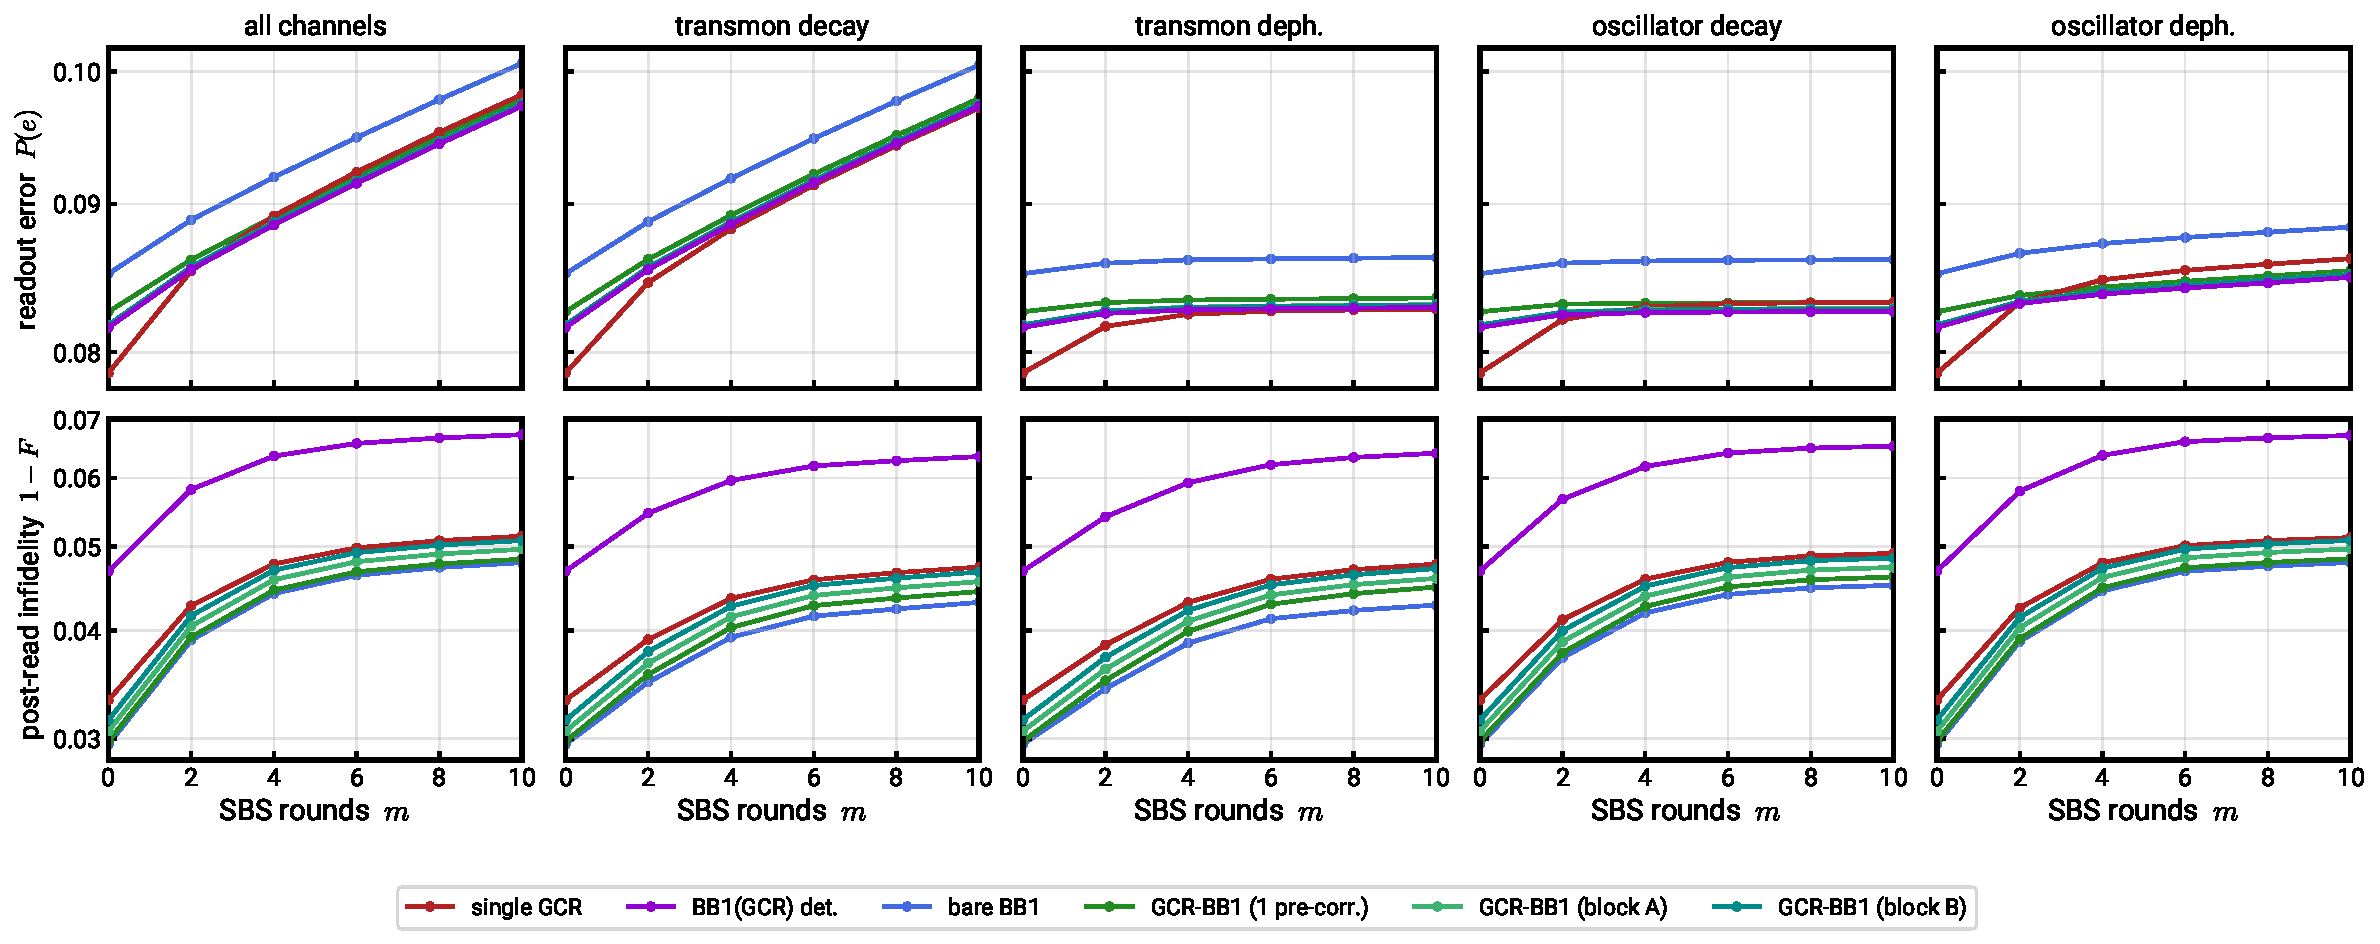
\includegraphics[width=\textwidth]{Paper_Figures/sbs_readout_sweep.pdf}
\caption{Reading an actively-stabilized logical~$0$ after $m$ rounds of \emph{noisy} SBS, under
\emph{noiseless} readout (isolating the stabilization noise). Columns are the five SBS-noise
conditions; top row is the readout error $P(e)$, bottom row the post-read oscillator infidelity
$1-F$; each panel overlays the six deterministic protocols versus the number of rounds $m$ (the
heralded scheme is omitted, see text). Note the linear vertical scale. All protocols share the
freshly-cooled floor at $m=0$ and rise gently; the rise is dominated by transmon decay (and the
all-channels case tracks it), while the oscillator channels and transmon dephasing are far
gentler. The protocol curves stay bunched within a few~$\times10^{-3}$ throughout.}
\label{fig:sbs}
\end{figure}

\begin{figure}[tbp]
\centering
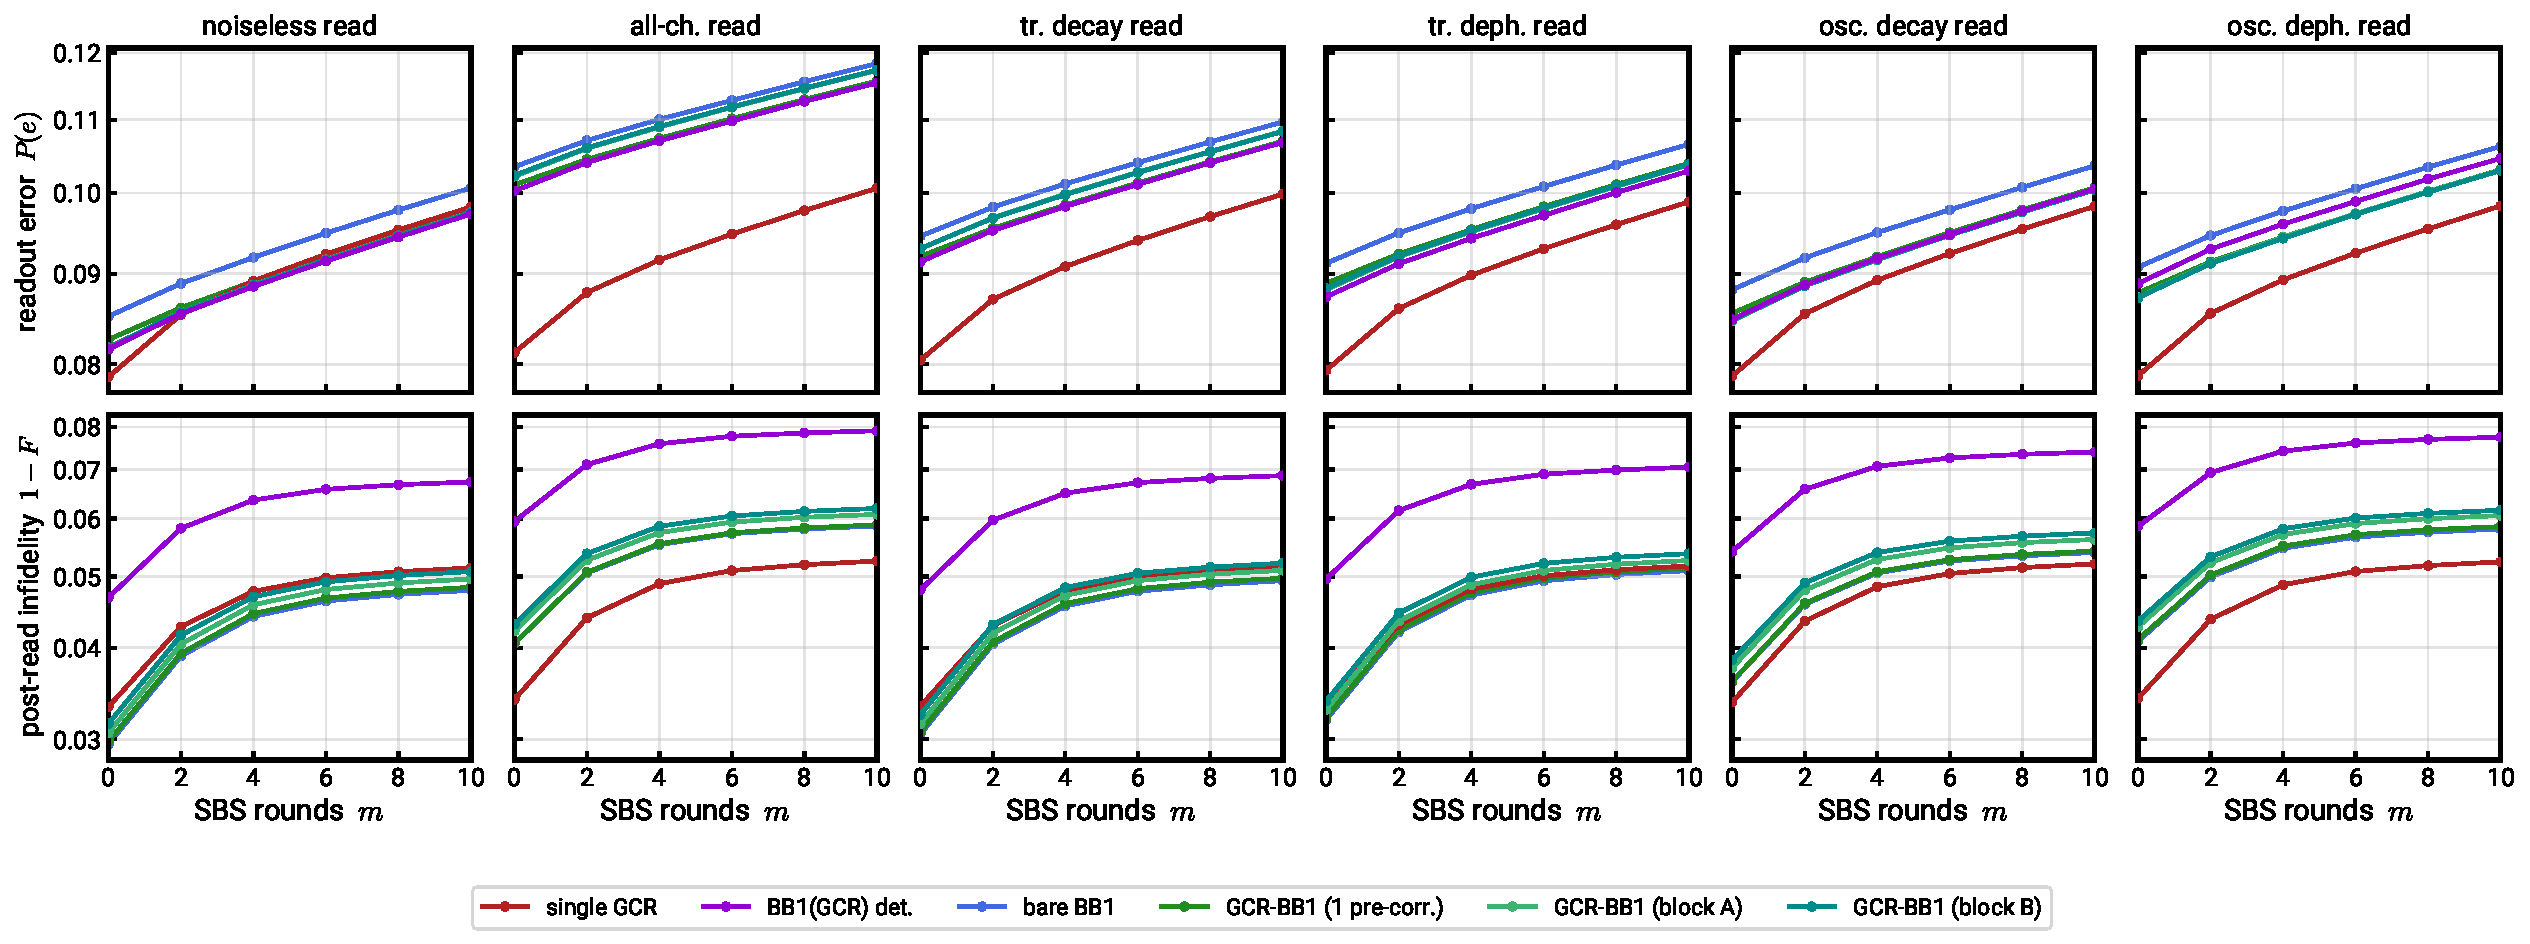
\includegraphics[width=\textwidth]{Paper_Figures/sbs_readout_conds.pdf}
\caption{The same experiment with the SBS stabilization fixed at its realistic all-channels
setting, now sweeping the \emph{readout}-circuit noise across its six conditions (columns). Rows
and curves as in Fig.~\ref{fig:sbs}. Readout noise shifts the $m$-dependence up by a nearly
constant, $m$-independent offset --- the two noise axes are separable --- largest for transmon
decay and the all-channels case, smallest for oscillator decay. The offset tracks circuit
\emph{duration}: single GCR (red), the shortest sequence, is almost immune and pulls clearly below
the five longer protocols, which lift together regardless of correction content --- reproducing the
short-circuit-wins verdict of Sec.~\ref{sec:damage}.}
\label{fig:sbs-readout}
\end{figure}

\paragraph{The state's-eye view, and the bottom line.} The oscillator infidelity
(bottom rows of Figs.~\ref{fig:sbs}--\ref{fig:sbs-readout}) tells the same story with one
addition. Starting from $1-F\in[0.030,0.047]$ at $m=0$, the post-read infidelity rises and then
\emph{saturates} beyond $m\approx4$: the noisy stabilizer reaches a fixed point at which entropy
injected per round balances entropy pumped out, so the state stops degrading rather than drifting
without bound. Here the protocol ordering does separate, and it \emph{inverts} between the two
metrics: bare BB1, which carries the \emph{largest} readout error of the six, nonetheless leaves
the \emph{most} faithful oscillator state ($1-F\approx0.048$ at $m=10$), while the detuning-heavy
BB1(GCR) correction --- among the best at pinning the readout bit --- leaves the \emph{least}
faithful state ($\approx0.067$). As in Sec.~\ref{sec:damage}, dressing the readout to sharpen the
logical bit comes at the cost of disturbing the oscillator it reads. Taken
together, the section's message is reassuring for the deterministic protocols: under realistic,
fully-noisy stabilization the readout error grows by only $\sim2\times10^{-2}$ over ten rounds and
the oscillator state saturates rather than collapses. The qualitative lessons of the earlier
sections thus carry over intact to a codeword that is being actively kept alive: readout-circuit
noise, not the readout construction, sets the achievable error, and the shortest state-relative
circuit is the most robust to it. What does \emph{not} carry over is any readout built around a
lattice-pinned measurement --- the heralded scheme, most accurate of all on pristine Gaussian-comb
codewords, cannot be pointed at the stabilized binomial codeword at all.
